\chapter{Лабораторная работа №3. LQR для линейного стационарного объекта}

\section*{Постановка (вариант 13)}
Дана система \(\dot x = A x + b u\), матрицы
\[
A=\begin{bmatrix}0&1\\4&3\end{bmatrix},\quad b=\begin{bmatrix}2\\6\end{bmatrix},\quad Q=\begin{bmatrix}6&0\\0&3\end{bmatrix},\quad r=2.
\]
Необходимо:
\begin{enumerate}
 \item Найти оптимальный регулятор \(u=-Kx\) на основе алгебраического уравнения Риккати (CARE)
 \[
  A^T P + P A - P b r^{-1} b^T P + Q = 0,\qquad K=r^{-1} b^T P.
 \]
 \item Смоделировать замкнутую систему \(\dot x=(A-bK)x\) при \(x(0)=[1,\,0]^T\), построить графики \(x_1, x_2, u, J(t)=\int_0^t (x^T Q x + r u^2)d\tau\), найти установившееся значение \(J(\infty)\).
 \item Незначительно изменить \(K\) (сохраняя устойчивость) и сравнить с оптимальным по критерию \(J\).
 \item Повторить моделирование для трёх значений \(r>0\) и \(Q_k=kQ\) (\(k>0\)), где для одного случая \(Q_k=Q\).
\end{enumerate}

\section{Решение CARE и формула регулятора}
Матрица \(b r^{-1} b^T = (1/r)\,b b^T\). Решая CARE для \(P\succ0\), получаем \(K=r^{-1} b^T P\). Далее проверяем устойчивость матрицы \(A-bK\) (собственные значения в левой полуплоскости). Численные значения приводятся ниже и воспроизводятся скриптом.

\subsection{Численная реализация}
\begin{lstlisting}[caption={LQR (вариант 13): решение CARE, моделирование и графики},label={lst:lqr13}]
# lab3/python/lqr_var13.py
import numpy as np
from scipy.linalg import solve_continuous_are, eigvals
from scipy.integrate import solve_ivp
import matplotlib.pyplot as plt

A = np.array([[0.0, 1.0],[4.0, 3.0]])
b = np.array([[2.0],[6.0]])
Q = np.array([[6.0, 0.0],[0.0, 3.0]])
r = 2.0

# CARE
P = solve_continuous_are(A, b, Q, r)
K = (1.0/r) * (b.T @ P)  # shape (1,2)
Acl = A - b @ K
print("K=", K)
print("eig(A-bK)=", eigvals(Acl))

# Cost integrand
def lqr_cost(x, u):
    return float(x.T @ Q @ x + r * u**2)

# Closed-loop dynamics and online cost accumulation
x0 = np.array([1.0, 0.0])
T = (0.0, 10.0)

def odefun(t, z):
    x = z[:2]
    u = - float(K @ x)
    jdot = lqr_cost(x, u)
    dx = (Acl @ x)
    return np.hstack([dx, jdot])

z0 = np.hstack([x0, 0.0])
sol = solve_ivp(odefun, T, z0, max_step=0.01, rtol=1e-8, atol=1e-10)

t = sol.t
x = sol.y[:2,:]
Jt = sol.y[2,:]
u = - (K @ x).ravel()

import os
os.makedirs('/home/leonidas/projects/itmo/optimal-control-theory/lab3/images/task3', exist_ok=True)

plt.figure(figsize=(6,4))
plt.plot(t, x[0], label='x1')
plt.plot(t, x[1], label='x2')
plt.xlabel('t'); plt.ylabel('states'); plt.grid(True, alpha=0.3)
plt.title('Closed-loop states')
plt.legend(); plt.tight_layout()
plt.savefig('/home/leonidas/projects/itmo/optimal-control-theory/lab3/images/task3/states.png', dpi=200)

plt.figure(figsize=(6,4))
plt.plot(t, u)
plt.xlabel('t'); plt.ylabel('u'); plt.grid(True, alpha=0.3)
plt.title('Control u(t)')
plt.tight_layout()
plt.savefig('/home/leonidas/projects/itmo/optimal-control-theory/lab3/images/task3/u.png', dpi=200)

plt.figure(figsize=(6,4))
plt.plot(t, Jt)
plt.xlabel('t'); plt.ylabel('J(0,t)'); plt.grid(True, alpha=0.3)
plt.title('Accumulated cost J')
plt.tight_layout()
plt.savefig('/home/leonidas/projects/itmo/optimal-control-theory/lab3/images/task3/J.png', dpi=200)

print({'J_final': float(Jt[-1])})
\end{lstlisting}

\begin{figure}[H]
    \centering
    \begin{subfigure}{0.48\textwidth}
        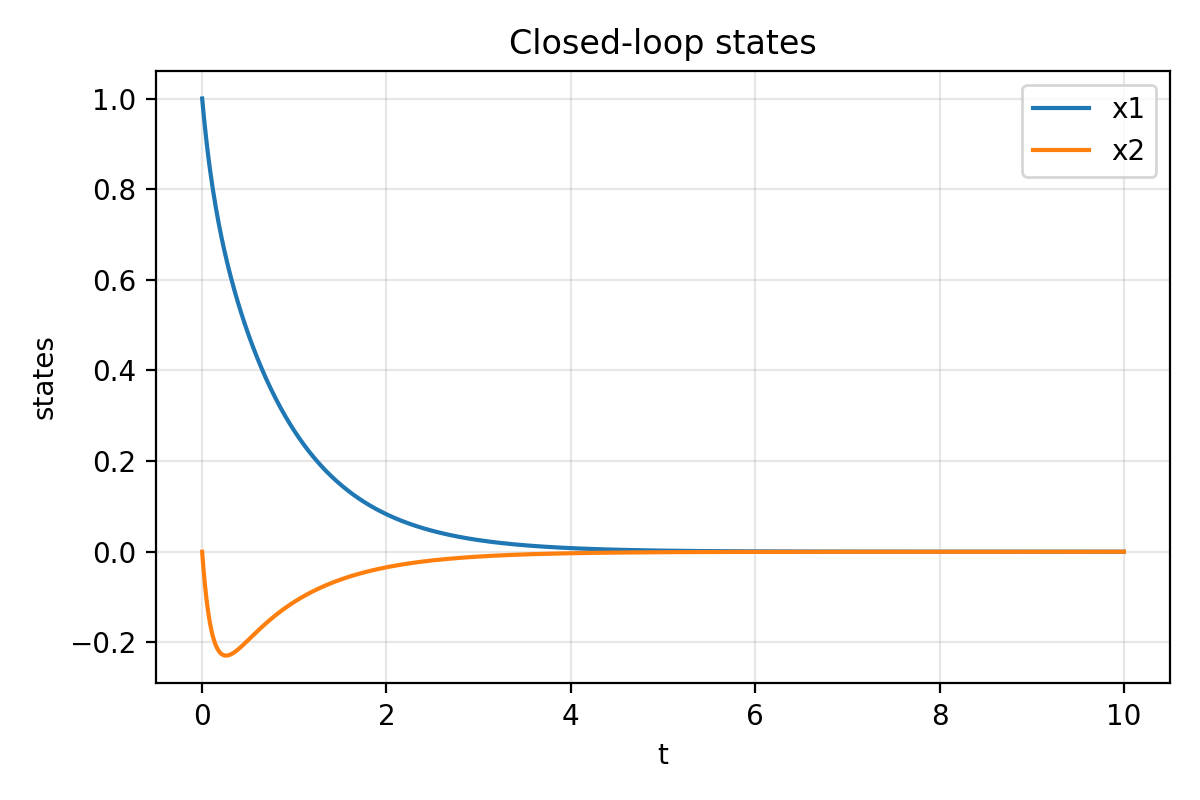
\includegraphics{task3/states.png}
        \caption{Состояния $x_1, x_2$}
    \end{subfigure}\hfill
    \begin{subfigure}{0.48\textwidth}
        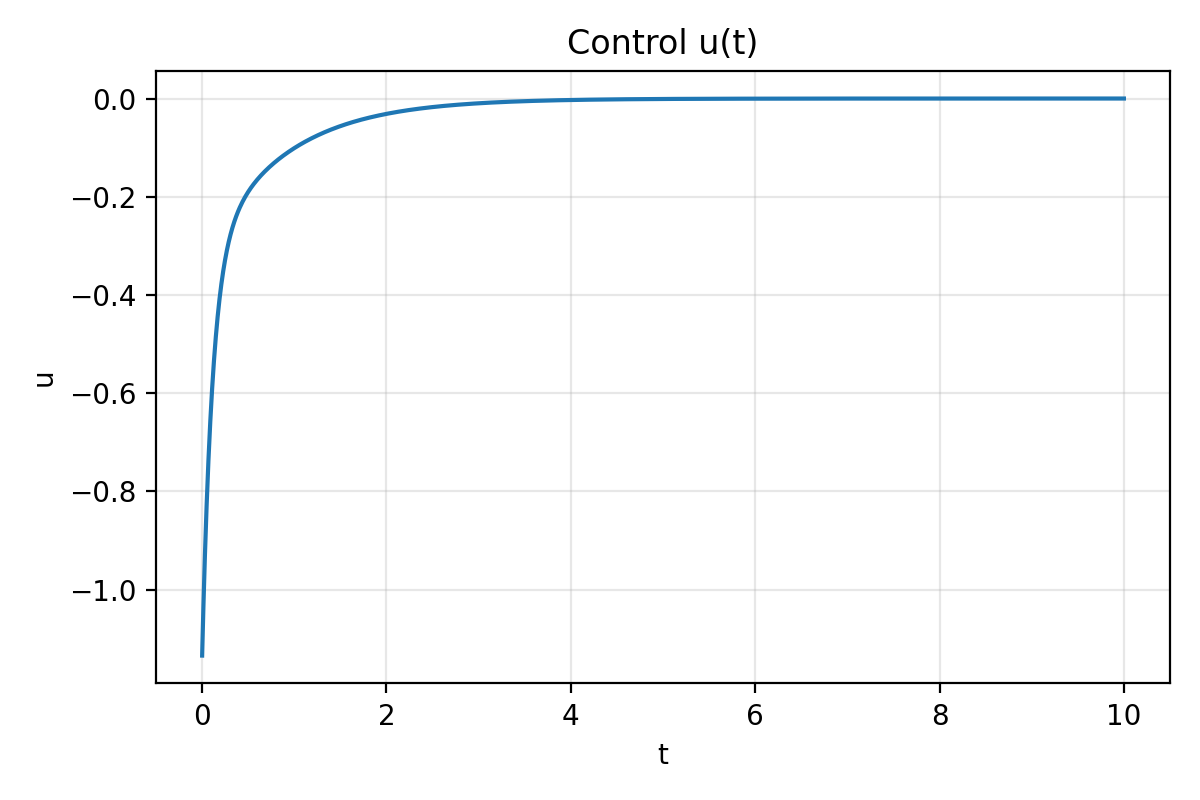
\includegraphics{task3/u.png}
        \caption{Управление $u(t)$}
    \end{subfigure}

    \vspace{0.5em}

    \begin{subfigure}{0.48\textwidth}
        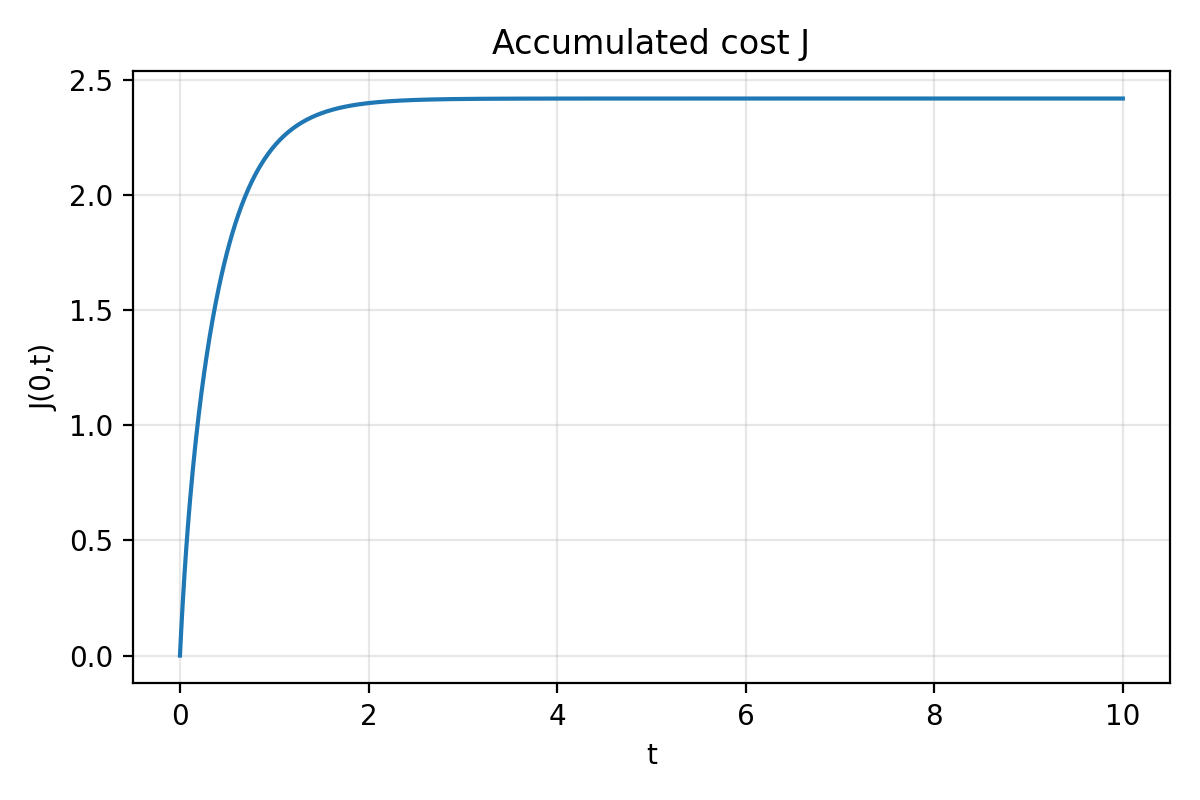
\includegraphics{task3/J.png}
        \caption{Накопленный критерий $J(0,t)$}
    \end{subfigure}
    \caption{LQR, вариант 13: моделирование замкнутой системы}
    \label{fig:l3:lqr}
\end{figure}

Для исходных параметров получено: \(K\approx[1.1345\; 1.8229]\), собственные значения \(A-bK\) равны \(-1.17\) и \(-9.03\) (устойчиво). Численно \(J(\infty)\approx 2.419\).
